\chapter{四波混频}
\label{ch:FWM}

由式~\ref{eq:average_power} 可知，单一频率光的平均功率随时间保持不变。若同时存在两个频率，它们的干涉会使平均功率随时间做正弦变化。由于 $\gamma\neq0$ 意味着折射率依赖于功率，因此两个频率同时存在于非线性介质中时，光场相位就会被周期性调制。这种过程会生成新的频率分量，称为“四波混频”（Four Wave Mixing, FWM）。




\section{电学相位调制}
为理解 FWM，先考虑一个连续波激光信号进入商用相位调制器，而该调制器由函数发生器输出的正弦电信号驱动。图~\ref{fig:PM} 给出了示意，实验演示可参考 \href{https://youtu.be/j8It3to54AQ}{这个视频}。输出信号满足
\begin{align}
    \label{eq:phase_modulator}
    \E_{out}&=\E_{in}\exp\left(i\Phi\cos(\omega_dT), \right)
\end{align}
其中 $\Phi$ 为调制器施加的最大相移，$\omega_d$ 为调制频率。关于这种调制对 $\E_{out}$ 实部的影响，可参考 \href{https://www.desmos.com/calculator/vcreo1gs2q}{这个交互图}。利用所谓的“Jacobi-Anger 展开”~\cite{NIST_JA_expansion}，式~\ref{eq:phase_modulator} 指数里的余弦项可写为
\begin{align}
\label{eq:JA}
    \exp\left(i\Phi\cos(\omega_dT)\right) &= \sum_{n=-\infty}^{\infty}i^n J_n(\Phi) \exp\left(in\omega_dT\right),
\end{align}
其中 $J_n(\Phi)$ 是第一类 $n$ 阶贝塞尔函数。简而言之，式~\ref{eq:JA} 表明：正弦相位调制会生成一系列新的、离散的频率分量，它们之间相隔 $\omega_d$，且各分量的相对功率取决于调制深度 $\Phi$。此外，把式~\ref{eq:chirp_definition} 用在式~\ref{eq:phase_modulator} 上可知，瞬时频率会随时间变化为 $\Phi\omega_d\sin(\omega_dT)$，这也再次说明相位调制本质上是在改变入射光的“颜色”。

\begin{figure}
    \centering
    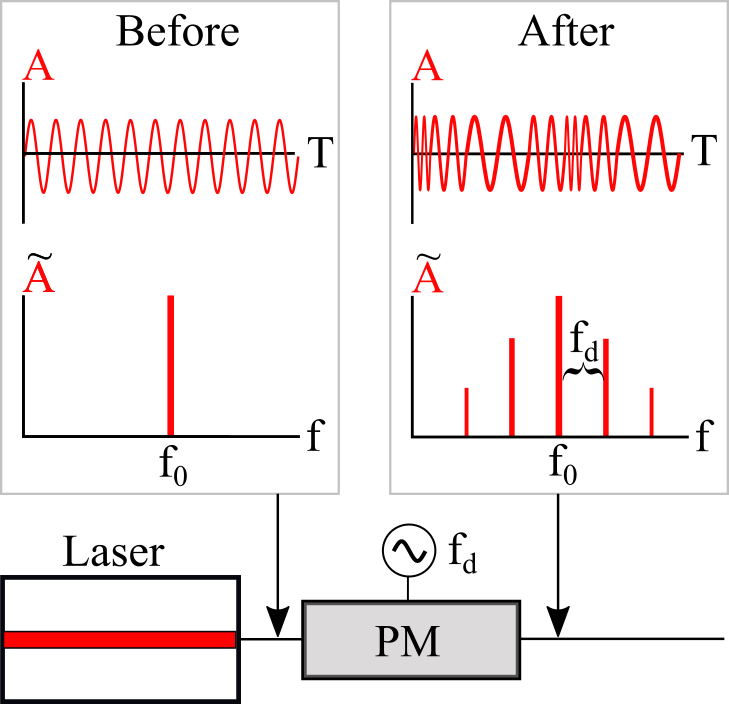
\includegraphics[width=1\linewidth]{figures/PhaseModulator.png}
    \caption{连续波光信号经过电学正弦相位调制后的示意图。进入调制器前，只有一个激光频率；经过调制器后，时域中交替出现的相位提前与延后等价于在频域中生成新的频率分量，这正是式~\ref{eq:JA} 所描述的内容。}
    \label{fig:PM}
\end{figure}

\section{基于非线性的相位调制}
\label{sec:sidebands}
下面这种 FWM 建模方式受到文献~\cite{Boskovic_Original_Kerr_Effect} 中原始推导的启发。考虑式~\ref{eq:SPM_applied}，并假设输入场 $\A(0,T)$ 可以写成两个连续波信号之和，它们的平均功率分别为 $P_a$ 与 $P_b$，频率间隔为 $\Delta\omega$：
\begin{align}
    \label{eq:FWM_input}
    \A(0,T)&= \sqrt{P_a}e^{-i\frac{\Delta\omega}{2}T}+\sqrt{P_b}e^{i\frac{\Delta\omega}{2}T}.
\end{align}
若输入实际上是有限时宽的两个脉冲，则连续波假设只是近似，但当 $\omega_d$ 大于脉冲本身带宽时，这个近似仍然有效。于是非线性介质末端的场为
\begin{align}
    \A(L,T) &= \A(0,T)\exp\left(i\gamma L [P_a+P_b+2\sqrt{P_aP_b}\cos(\omega_dT)] \right) \\ \nonumber
    &= \A(0,T)\exp\left(i\gamma L [P_a+P_b]\right)\exp\left(i2\gamma L\sqrt{P_aP_b}\cos(\omega_dT) \right)\\ \nonumber
    \A(L,T)Q^{-1}&= \A(0,T)\exp\left(i2\gamma L\sqrt{P_aP_b}\cos(\omega_dT) \right)\\ \nonumber
    \A(L,T)Q^{-1}&= \A(0,T)\exp\left(i\phi_{NL}\cos(\omega_dT) \right),
\end{align}
其中为方便起见，把与时间无关的因子 $Q=\exp(i\gamma L [P_a+P_b])$ 暂时移到等式左边。再应用式~\ref{eq:JA} 得到
\begin{align}
    \A(L,T)Q^{-1}&= \A(0,T)\sum_{n=-\infty}^{\infty}i^nJ_n(\phi_{NL})e^{in\omega_dT} \\ \nonumber
    &=\left(\sqrt{P_a}e^{-i\frac{\Delta\omega}{2}T}+\sqrt{P_b}e^{i\frac{\Delta\omega}{2}T}\right)\sum_{n=-\infty}^{\infty}i^nJ_n(\phi_{NL})e^{in\omega_dT} \\ \nonumber
    &=\sqrt{P_a}\sum_{m=-\infty}^{\infty}i^mJ_m(\phi_{NL})e^{i\left(m-\frac{1}{2}\right)\omega_dT}+...\\ \nonumber & \quad\quad\quad\quad\quad\sqrt{P_b}\sum_{k=-\infty}^{\infty}i^kJ_k(\phi_{NL})e^{i\left(k+\frac{1}{2}\right)\omega_dT}.
\end{align}
注意，这里把原本以 $n$ 为索引的一个无穷和拆成了分别以 $m$ 和 $k$ 为索引的两个无穷和，因为 $\A(0,T)$ 中的两个复指数项会把对应频率整体平移，导致“第一组中 $m=1$ 的频率”与“第二组中 $k=1$ 的频率”并不相同。为重新合并这两个求和，可令 $m=k+1$，从而得到
\begin{align}
\label{eq:re_index}
    \A(L,T)Q^{-1}&=\sqrt{P_a}\sum_{k=-\infty}^{\infty}i^{k+1}J_{k+1}(\phi_{NL})e^{i\left(k+\frac{1}{2}\right)\omega_dT}+...\\ \nonumber & \quad\quad\quad\quad\quad\sqrt{P_b}\sum_{k=-\infty}^{\infty}i^kJ_k(\phi_{NL})e^{i\left(k+\frac{1}{2}\right)\omega_dT} \\ \nonumber
    &= \sum_{n=-\infty}^{\infty} i^n\left[i\sqrt{P_a}J_{n+1}\left(\phi_{NL}\right)+\sqrt{P_b}J_n\left(\phi_{NL}\right)\right]e^{i\omega_d\left(n+\frac{1}{2}\right)T}.
\end{align}
最后再把 $Q$ 移回等式右边，得到
\begin{align}
\label{eq:FWM_general}
    \A(L,T)&=\sum_{n=-\infty}^{\infty} i^n\left[i\sqrt{P_a}J_{n+1}\left(2\gamma L\sqrt{P_aP_b}\right)+\sqrt{P_b}J_n\left(2\gamma L\sqrt{P_aP_b}\right)\right]e^{i\omega_d\left(n+\frac{1}{2}\right)T+i\gamma L[P_a+P_b]}.
\end{align}
在式~\ref{eq:FWM_general} 中，$n=-1$ 对应的频率分量位于 $-\omega_d/2$，$n=0$ 对应的分量位于 $+\omega_d/2$，这两项正好对应式~\ref{eq:FWM_input} 中原本的两个输入频率。第 $n$ 阶边带的平均功率为
\begin{align}
\label{eq:sideband_power}
    |\A_n(L,T)|^2 &= P_aJ^2_{n+1}\left(2\gamma L \sqrt{P_aP_b}\right)+P_bJ^2_{n}\left(2\gamma L \sqrt{P_aP_b}\right).
\end{align}
关于不同 $2\gamma L \sqrt{P_aP_b}$ 下边带功率的数值模拟，见图~\ref{fig:FWM}a) 和 b)；图~\ref{fig:FWM}c) 给出了数值结果与式~\ref{eq:sideband_power} 预测之间的比较。若进一步假设 $P_a\ll P_b$ 且 $2\gamma L\sqrt{P_aP_b}<\sqrt{1+n}$（其中 $n>0$），则有
\begin{align}
\label{eq:sideband_approx}
    |\A_n(L,T)|^2 &\approx P_b\frac{(\gamma^2 L^2P_aP_b)^{n}}{n!^2},
\end{align}
因为当自变量较小时，贝塞尔函数满足
\begin{align}
\label{eq:Bessel_approx}
    J_n(x)&\approx \frac{1}{n!}\left(\frac{x}{2}\right)^n.
\end{align}
图~\ref{fig:FWM}d) 展示了式~\ref{eq:sideband_approx} 所预测的这种缩放关系。高阶边带功率对输入功率的变化比低阶边带更敏感，这一性质在多种全光信号处理技术中都很有用~\cite{my_thesis,BenoitPhD,YangLuPhD}。若想看一种同时考虑色散的 FWM 建模方式，可参考 \href{https://youtu.be/0SXPvO89jto}{这个教程视频}；实验演示可见 \href{https://youtu.be/gsa9hrCbnqI}{这个视频}。
\begin{figure}
    \centering
    
\includegraphics[width=1.0\linewidth]{figures/FWM_combined.png}
    \caption{a) 两个相隔 5~GHz、满足 $P_b=100P_a$ 的频率分量在非线性介质中传播，当 $\phi_{NL}=2\gamma L\sqrt{P_aP_b}=1.08$~rad 时，数值计算得到的初始与末端频谱。注意：较强频率的功率转移到邻近边带，同时边带阶数越高功率下降越快，这与式~\ref{eq:sideband_approx} 一致。b) 与 a) 相同，但取 $\phi_{NL}=7.2$~rad。c) 归一化到 $P_b$ 后的边带功率，比较数值模拟与式~\ref{eq:sideband_power} 的结果。d) 与 c) 类似，但在双对数坐标中对 $\phi_{NL}$ 作图，以展示式~\ref{eq:sideband_approx} 预测的缩放行为。这些图由 \href{https://colab.research.google.com/drive/1l054EDg-50aK5GORN_md4_-tlFy4jwC5?usp=sharing}{这个交互式 notebook} 生成。}
    \label{fig:FWM}
\end{figure}

\section{交叉相位调制（XPM）}
\label{Sec:XPM}
在第~\ref{ch:SPM} 章中我们已经看到：单一频率光场在非线性介质中的相位会随其平均功率线性增加。当同时存在两个频率分量时，可由式~\ref{eq:FWM_general} 计算其中一个频率分量的相位如何同时依赖于自身平均功率以及另一个频率分量的平均功率。取其中 $n=0$ 的项，有
\begin{align}
    \phi_0 &= \frac{\omega_d}{2}T+\gamma L [P_a+P_b]+\theta_0,
\end{align}
其中
\begin{align}
\label{eq:theta}
    \theta_0 &= arg\left( i\sqrt{P_a}J_{1}\left(2\gamma L\sqrt{P_aP_b}\right)+\sqrt{P_b}J_0\left(2\gamma L\sqrt{P_aP_b}\right) \right) \\ \nonumber
    &= \arctan\left(\frac{\sqrt{P_a}J_{1}\left(2\gamma L\sqrt{P_aP_b}\right)}{\sqrt{P_b}J_0\left(2\gamma L\sqrt{P_aP_b}\right) } \right).
\end{align}
利用式~\ref{eq:Bessel_approx}，可把式~\ref{eq:theta} 近似写成
\begin{align}
    \theta_0 &\approx\arctan\left(\frac{\sqrt{P_a}\gamma L\sqrt{P_aP_b}}{\sqrt{P_b} } \right) \\ \nonumber
    &\approx\arctan\left(\gamma LP_a\right) \\ \nonumber
    &\approx \gamma LP_a.
\end{align}
于是，第 $n=0$ 个频率分量的相位可写作
\begin{align}
    \label{eq:XPM}
    \phi_0 &\approx \frac{\omega_d}{2}T+\gamma L [P_a+P_b]+\gamma LP_a \\ \nonumber
    &=\frac{\omega_d}{2}T+\gamma L [2P_a+P_b].
\end{align}
注意，$n=0$ 对应的频率位于 $+\omega_d/2$，它在初始时的平均功率就是 $P_b$。因此式~\ref{eq:XPM} 中含 $P_b$ 的那一项对应 SPM，而含 $P_a$ 的那一项则对应所谓的“交叉相位调制”（Cross Phase Modulation, XPM）。有意思的是，式~\ref{eq:XPM} 表明 XPM 的强度约为 SPM 的两倍，这一点在图~\ref{fig:XPM} 的数值模拟中得到了验证。关于从麦克斯韦方程出发推导 XPM 的另一种方法，可参考 \href{https://youtu.be/aDXd13zLPC4}{这个视频教程}；若想看 SPM 与 XPM 相对作用的可视化示例，可参考 \href{https://www.desmos.com/calculator/vstlwgtlyb}{这个交互图}。

\begin{figure}
    \centering
    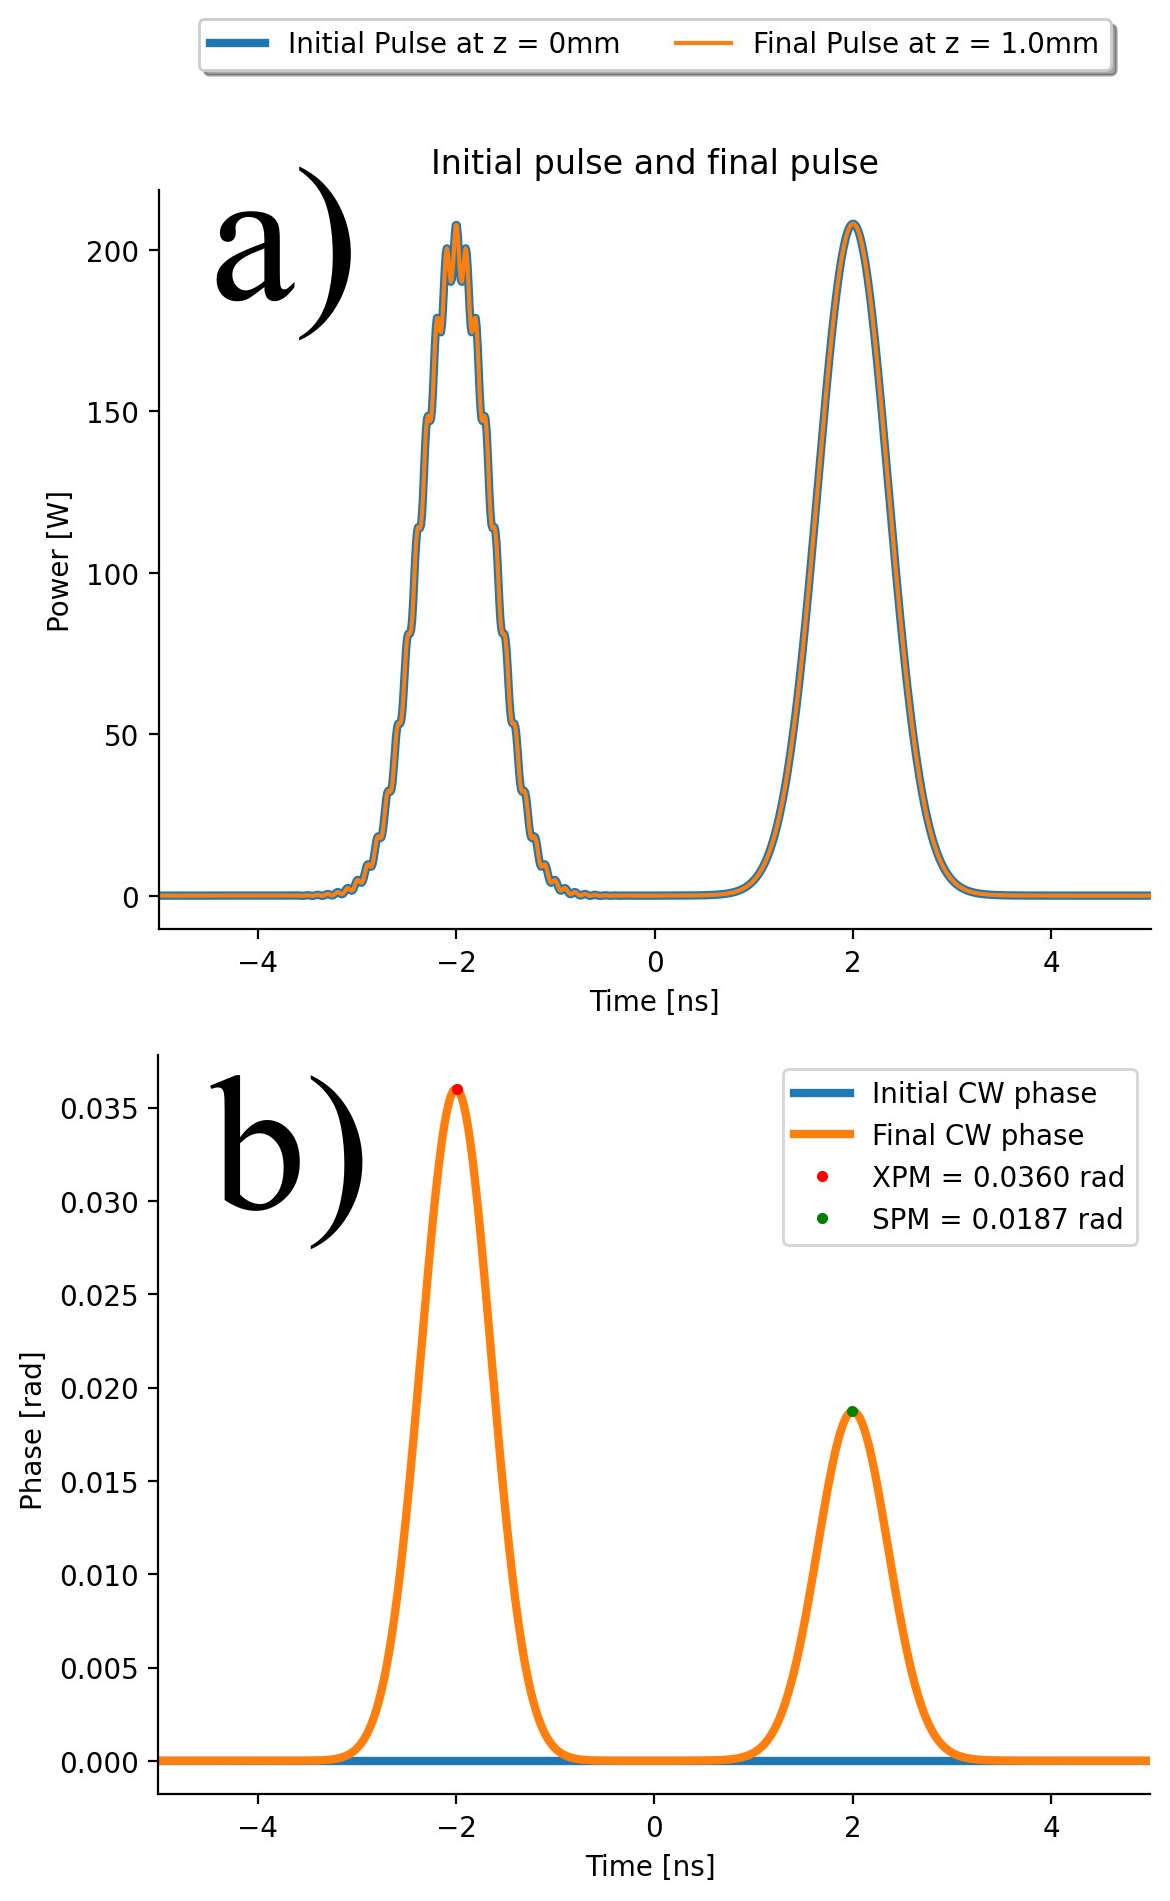
\includegraphics[width=0.8\linewidth]{figures/XPM_combined.png}
    \caption{SPM 与 XPM 对光信号相位作用强弱不同的示意图。a) 时域中，一个低功率连续波信号与两个高功率高斯脉冲重叠，两个脉冲唯一差别是载波频率不同。左侧脉冲的载波频率比连续波低 10~GHz。b) 在非线性介质中传播后，连续波从 XPM 获得的相移约为 SPM 的两倍，这与式~\ref{eq:XPM} 一致。图中 $0.0360/0.0187\approx 1.925\neq2$ 的偏差来自式~\ref{eq:XPM} 中的近似以及有限的数值时间分辨率。这些图由 \href{https://colab.research.google.com/drive/1aIRradfOZGN7JYUhbtYJdVzJwAZoYoUe?usp=sharing}{这个交互式 notebook} 生成。}
    \label{fig:XPM}
\end{figure}






\section{相位匹配}
\label{sec:Phase_matching}
第~\ref{sec:sidebands} 节的推导默认色散可以忽略，这适用于 $\omega_d$ 足够小、且载波频率靠近第~\ref{subsec:ZDF} 节所述零色散频率的情形。关于色散对 FWM 的影响，可参考 \href{https://youtu.be/0SXPvO89jto}{这个视频教程}。结论是：当 $\betag_2>0$ 时，FWM 较弱；而在满足
\begin{align}
\label{eq:phase_matching}
0&=\betag_2\omega_d^2+\gamma(P_a+P_b)    \\ \nonumber
\betag_2&=-\gamma(P_a+P_b)/\omega_d^2<0,
\end{align}
时，FWM 最强。这里默认 $\omega_d$ 足够小，以至于式~\ref{eq:beta_approx} 中只有 $\betag_2$ 需要保留。其原因在于，FWM 本质上是一个\emph{相干}过程：输入电磁波先把功率相干地转移到非线性介质折射率的振荡变化上，再由后者相干地转移到另一组电磁频率。简而言之，非线性会使入射光驱动介质中那些微小偶极子以新的时间频率振荡；如果其中某个振荡对应的空间频率，恰好与另一束电磁波的空间频率一致，那么该波的功率就会像 \href{https://youtu.be/bha8SzWzRc4}{这个视频教程} 所解释的那样，因相长干涉而随传播距离增加。式~\ref{eq:phase_matching} 中的条件正是由此而来：新波与入射波之间的空间频率失配必须很小，而初始场功率引起的折射率增加又会把空间频率推大，因此需要一个负的 $\betag_2$ 去补偿。这种“介质常规折射率引起的空间频率变化”与“场功率通过非线性引起的空间频率变化”彼此平衡的现象，就称为“相位匹配”。式~\ref{eq:phase_matching} 是 FWM 这一特例的相位匹配条件，对本教程范围之外的其他非线性过程，也能写出类似关系，例如 \href{https://www.youtube.com/watch?v=UpuN0dS23Nw}{二次谐波产生}、\href{https://youtu.be/bha8SzWzRc4}{三次谐波产生} 和 \href{https://www.creol.ucf.edu/mir/wp-content/uploads/sites/7/2023/07/L22_-Stimulated-Brillouin-scattering.pdf}{受激布里渊散射}。

\subsection{调制不稳定性}
FWM 的一个直接后果是：若某个非线性介质在某载波频率处满足 $\betag_2<0$，则信号在向前传播的过程中会变得更嘈杂。原因是载波与电磁场中微弱而无处不在的涨落之间会产生干涉，从而通过 FWM 把光功率从载波转移到邻近频率上，如 \href{https://prefetch.eu/know/concept/modulational-instability/}{这里} 所解释并由图~\ref{fig:MI} 所示。某些噪声频率因满足相位匹配而被优先放大的过程，称为“调制不稳定性”（Modulation Instability, MI）。更多细节可见 \href{https://youtu.be/VtaoPd0Fwj8}{这个视频教程}。

\begin{figure}
    \centering
    
\includegraphics[width=0.75\linewidth]{figures/MI_combined.png}
    \caption{a) 一个由高斯脉冲与随机噪声组成的信号，在具有 $\betag_2<0$ 的非线性介质中传播 100~m 前后的时域功率，其中噪声幅度比高斯脉冲小 1000 倍。b) 与 a) 对应的频谱。c-d) 分别对应传播 200~m 的时域和频域结果。e-f) 分别对应传播 300~m 的结果。g) 传播 500~m 时的完整时域演化。h) 对应的频谱演化。这些图由 \href{https://colab.research.google.com/drive/1p2aQZ4zPPAIMplVxvlezdmpQt_j-rsY7?usp=sharing}{这个交互式 notebook} 生成。}
    \label{fig:MI}
\end{figure}
